\section{Syntax-Aware On-the-Fly Code Completion}\label{sec:approach}


In this section, we present an overview of our syntax-aware on-the-fly Python code completion approach (\our).

Conceptually, \our~aims to generate source code at any time regardless of the completeness of the source code, while considering the syntactic and semantic information of the source code during the learning phase, but \emph{do not} require syntactic information during the inference phase.
To ensure that the learning process considers both semantic and syntactic information, we design our approach to focus on two prediction tasks, i.e., the code token prediction task and the token type prediction task.
In particular, we leverage a Multi-Task Training technique (MTT) to cooperatively learn both the code token prediction task (Task 1: Predict the next code token, considered as a Target Task) and the token type prediction task (Task 2: Predict its token type, considered as a Supporting Task).
For the type prediction task, we propose to leverage the standard Python token type information (e.g., String, Number, Name, Keyword), which is readily available and lightweight, instead of using the AST information~\cite{kim2021code, izadi2022codefill, li2017code, svyatkovskiy2019pythia, liu2020self, liu2022unified} where we found not available for the two-third of the executions (see our finding in Section~\ref{sec:motivation}), limiting its ability to perform on-the-fly code completion.
In contrast, our \our~\emph{does not} require syntactic information at the inference phase.
Thus, the completeness of the source code at the inference time is not required.


% , 
% we found 


% Unlike some previous work that leverages AST information as an individual learning objective for the AST node prediction task~\cite{kim2021code,li2017code},
% Our research study on how to best use this token type information along with source code.
% To ensure that our model captures both syntactic and semantic information during the learning process, we leverage Multi-Task Learning (MTL) techniques to simultaneously learn both the token prediction task and the type prediction task. 



% \textit{Finish}  \kla{please add some key general principles. what is the model? how does the model work? what is the learning objective of the model? how does this model differ from others? why new data collection is needed? what existing dataset is not enough to be used? so we need to perform the following three steps}

% In this section, we present an overview of our approach, \emph{SynComp}, a multi-task training model which learns semantic and syntactic information cooperatively.
% % which learn semantics information via source code, and light-weight syntactic information via token types.
% \kla{should we talk about two prediction tasks somewhere? Task1=? and Task2=}
% The model learn a semantic information from source code which does not require the completeness (i.e. on-the-fly); 
% and apply a token type information to solve the limitation (section 2.2) and learn a light-weight syntactic information (i.e. syntactic-aware).
% Thus, SynComp training phase consists of 2 tasks: source code prediction (target task) and token type prediction (supporting task).
% In order to train the model to learn on multiple task simultaneously, 
% The supporting task (a.k.a. an auxiliary task) is a non-target task that help improve the performance of the target task.
% There are variety techniques on training multi-task SynComp leverage Multi-Task Learning (MTL) and Intermediate Fine-tuning (STILTs) techniques in this work.
% Such techniques have different way

% SynComp leverages Byte-Pair-Encoding (BPE) method~\cite{sennrich2015neural} to handle new unseen tokens; leverages MTL and STILTs~\cite{weller2022use} to address multiple tasks training challenge; and explores varieties of task weighing parameters and decoding methods to find the best perform architecture for code completion.

% In this section, we present an overview of our approach, \emph{SynComp}, a Syntactic-Aware On-the-Fly Code Completion model that learn to complete code with the knowledge enhancement in syntactic information by token types.
% Pure source code sequential model (e.g. CodeGPT and GPT-2) learn semantics data from source code. 
% However, with the support of auxiliary task, i.e. the non-target task which help improve the performance of primary task, such as token type information, SynComp picks up both semantics and syntactic information. 

\textbf{Overview.} Figure~\ref{fig:overview} presents the overview of our \our, which consists of two phases: training and inference.
During the training phase, \our~performs 6 main steps:
Step~\circled{1} Type Extraction, to extract the token type information from source code;
Step~\circled{2} Tokenization, to perform subword tokenization on the source code;
Step~\circled{3} Data Alignment, to align the type information which is word level to the code information which is currently subword level;
Step~\circled{4} Multi-task Training Architecture with 3 training techniques: hard parameters sharing (MTL), soft parameters sharing (MTL), and intermediate fine-tuning (IFN);
then in Step~\circled{5} Hyperparameter Task Weighing and Step~\circled{6} Decoding Methods are the exploration steps to maximize the performance.
For the inference phase, we describe in Step~\circled{7} Code Generation step in the details of token-level prediction and line-level prediction.
% Below, we present the details of each step.

% \textbf{Problem Formulation.} 
% We perform the experiments on 2 kinds of completion level: token-level prediction and line-level prediction.

% MTL - Hard/Soft
% IFT - STILTs

% First, in \emph{(3.1) Data Collection} we extract the token type information from the source code. Then, in \emph{(3.2) Data Processing}, we tokenize the source code with \gls{bpe} algorithm and align the type information to the sub-words. Thus, the training phase consist of 2 tasks: source code prediction and token type prediction. In \emph{(3.3) Model Architectures}, we proposed 3 training techniques: hard parameters sharing MTL, soft parameters sharing MTL, and intermediate fine-tuning. For the inference phase, the model predict the task separately requiring no additional data for each task. Following is the details of our approach.

% We describe our approach in this session. Firstly, we elaborate how we collect the type dataset. Then since our model use BPE tokenizer, we align the type dataset to our source code to be in the same sequences. Lastly, we describe the models experiments which consist of 3 kinds: hard parameters sharing model, soft parameters sharing model, and intermediate fine-tuning model.

\begin{figure*}
    \centering
    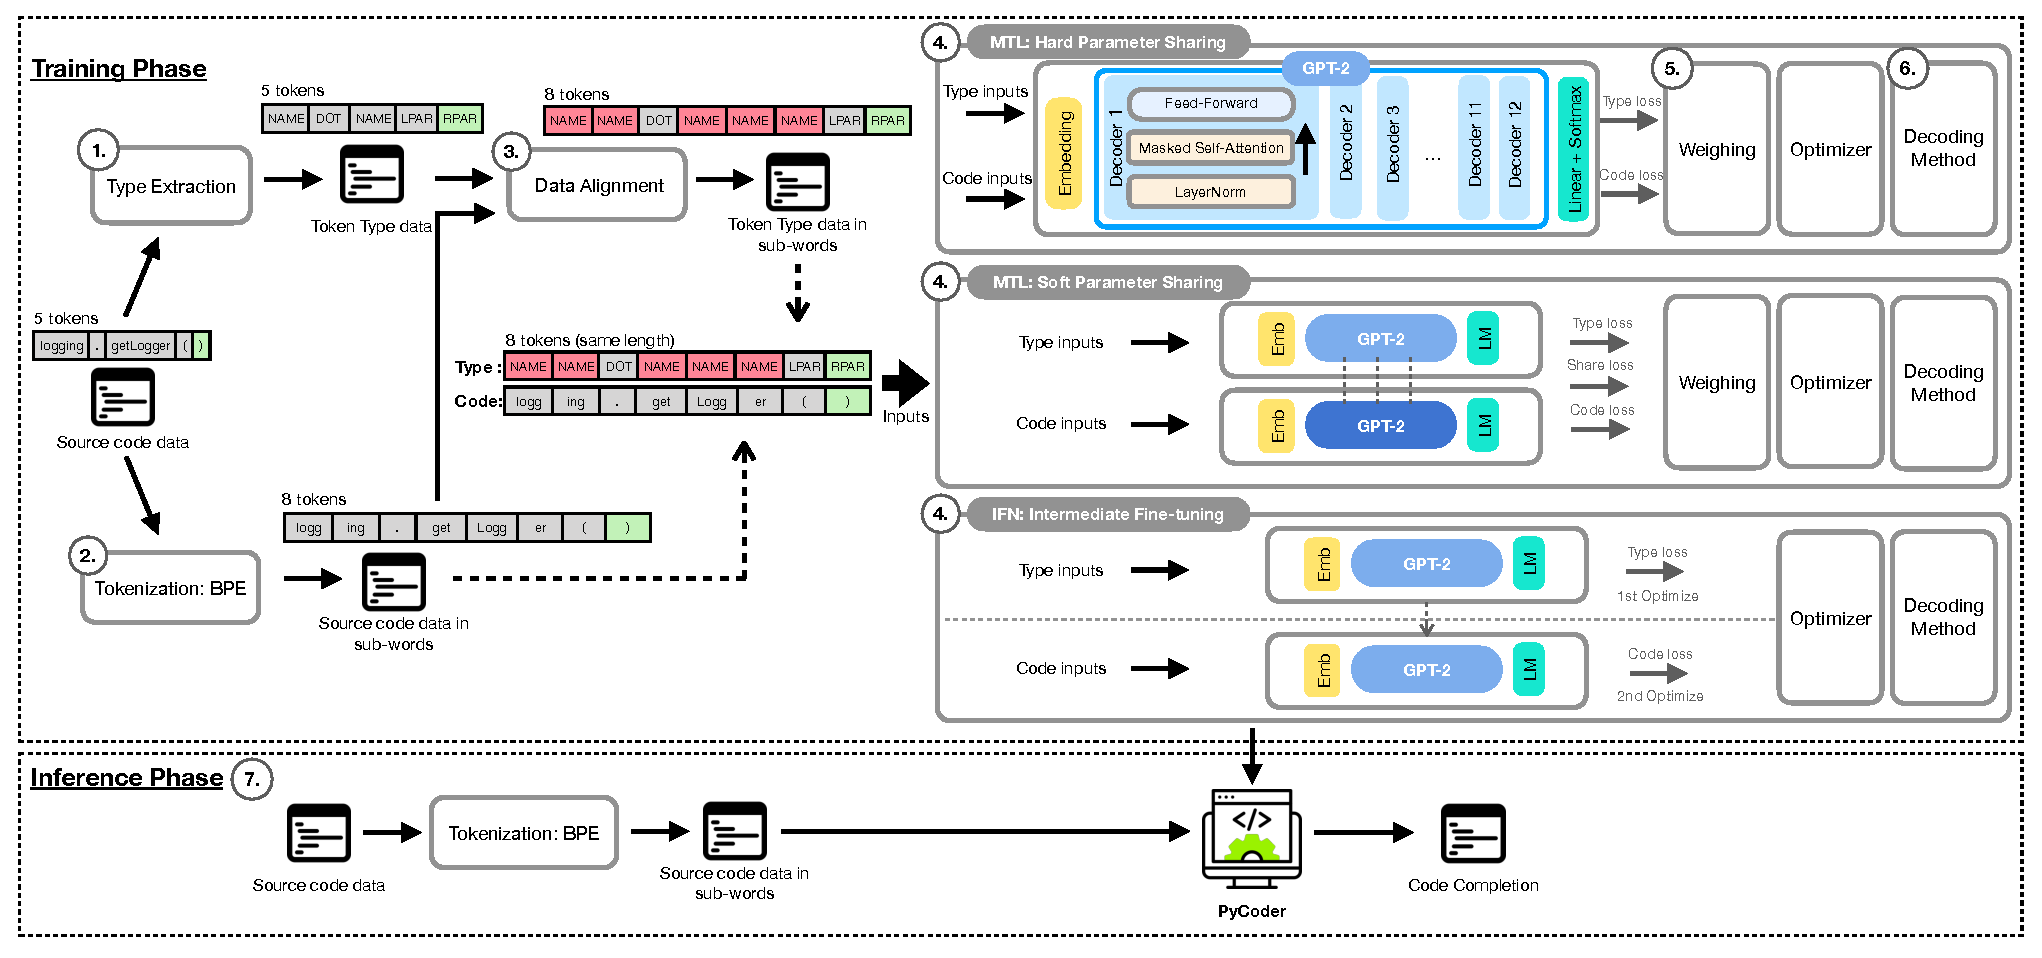
\includegraphics[width=\textwidth]{figures/overview.pdf}
    \caption{
    % \kla{An} \kla{o}verview of our \kla{syntactic-aware on-the-fly code completion} approach (\kla{SynComp})\kla{.} \kla{add a full stop in the caption everytime.} \kla{remove tag when reading this one.} \kla{This figure is nicely presented. Well done! Looks very neat.}
    An overview of our Syntax-Aware On-the-Fly Python Code Completion approach (PyCoder). 
    % \kla{can you use 1,2,3 instead of 3.1, 3.2, 3.3? Thank you.}
    }
    \label{fig:overview}
\end{figure*}

\subsection{(Step 1) Type Extraction}

Syntactic information can be represented in many forms, e.g., Abstract Syntax Tree (AST) which is widely used in the previous work, and Token Type information which remains largely unexplored.
In fact, both AST and token type information have their own advantages and disadvantages.
While AST provides a formal representation of syntactic information of source code, it requires syntactically correct source code in order to be successfully parsed by a Python AST parser.
Since our finding in Section~\ref{sec:motivation} shows that the Python AST parser failed to execute for every two out of three characters that developers type, the usage scenarios of the existing AST-based code completion approach are still limited in practice.

To address this challenge, we leverage a standard Python token type information, offering a more abstract representation of the syntactic structure of source code (e.g., Name, String, Number), which (1) is more lightweight, (2) follows the natural order of code sequences; and (3) can be successfully parsed at any times without requiring the complete and syntactically correct source code.
Generally, the standard Python token consists of two pieces of information i.e., (1) the token type, which provides syntactic meaning, and (2) the token value, which provides semantic meaning.
% Thus, each token is a substring that has semantic meaning in the grammar of the Python programming language.\footnote{https://www.asmeurer.com/brown-water-python/intro.html}
For example, given a \texttt{logging} token, the token type is \texttt{NAME} and its value is \texttt{logging}.
Since the token type information is not available in the existing code completion benchmark, we describe the steps to extract the type information below.





% The definition of a token for this tokenizer is a substring that has semantic meaning in the grammar of python language 4; thus, every token extracted by this tokenizer has a type (i.e. token type)








% To address the limitation, the token type information from a standard python tokenizer is leveraged in this work. The definition of a token for this tokenizer is a substring that has semantic meaning in the grammar of python language 4; thus, every token extracted by this tokenizer has a type (i.e. token type). Unlike AST, this token type information can be extracted at any points in source code, and can handle the invalid source code. Only the case that user has not finished typing the whole last word that the type information of the last word could return incorrectly. However, the rest of the token type information will still be able to accurately achieve






% - token type - pros - lightweight - abstracted 
% cons - not syntactically correct guaranteed like AST when generate
% - natural order of source code 


% While AST provides a formal representation of 


% AST - type and value

% correct type, wrong value -> generated code is syntactically correct, but incorrect predictions

% incorrect type, correct value -> generated code is (i.1 instead of i=1) due to incorrect type prediction.


% - AST  - cons - it requires syntactically correct source code all the time.
% - pros, generate syntactically correct nodes all the time

% given source code-> code to AST -> AST is fed into the model -> model learn to generate a new node -> producing a tree with a new node -> this tree can be parsed back to a sequence of source code, for code completion - 

% code and AST is inter-parsability

% 2/3 --- failed

% incorrect node prediction -> wrong tree -> wrong code completion

% correct node prediction, incorrect value prediction -> correct tree, but wrong code, but executable.










% Type information plays an important role in teaching model to learn the syntactic information.
% Since the benefit behind the types is to categorize the unstructured data of natural text in source code (e.g. different variable naming) into discrete groups.
% These discrete groups arranged together in sequences could represent the structures of source code, i.e. syntactic information.
% In previous works, AST type has been widely used for syntactic information; however, as discussed earlier  (section 2.2), AST is not on-the-fly information.

% To address the limitation, the token type information from a standard python tokenizer is leveraged in this work.
% The definition of \emph{a token} for this tokenizer is a substring that has semantic meaning in the grammar of python language~\footnote{https://www.asmeurer.com/brown-water-python/intro.html}; thus, every token extracted by this tokenizer has a type (i.e. token type).
% Unlike AST, this token type information can be extracted at any points in source code, and can handle the invalid source code.
% Only the case that user has not finished typing the whole last word that the type information of the last word could return incorrectly. 
% However, the rest of the token type information will still be able to accurately achieve.


To extract type information, we use the \texttt{tokenizer} function provided by the standard Python tokenizer library\footnote{https://docs.python.org/3/library/tokenize.html} with an option \texttt{exact\_type} in order to extract the most fine-grained type for each token.
For the Python tokenizer (Python 3.7 version), there will be a total of 58 different types.
In particular, we focus on the 12 primary types of code tokens as follows: \texttt{<NAME>}, \texttt{<NUMBER>}, \texttt{<STRING>}, \texttt{<INDENT>}, \texttt{<DEDENT>}, \texttt{<ERRORTOKEN>}, \texttt{<ENDCODING>}, \texttt{<ENDMARKER>}, \texttt{<COMMENT>}, \texttt{<NL>}, \texttt{<NEWLINE>}, and \texttt{<OP>}, where the \texttt{<OP>} type consists of the remaining 46 operational types (e.g., operator. delimiter), such as \texttt{<LESS>}, \texttt{<GREATER>}, \texttt{<EQUAL>}, \texttt{<DOT>}.
Then, we perform the following pre-processing steps.

\begin{itemize}
    \item First, we discard the following three token types that will not be executed, i.e., \texttt{<ENCODING>} which describes the encoding of the Python file, \texttt{<ENDMARKER>} which describes the end position of the Python file, and \texttt{<COMMENT>} which describes the code comment of the Python file.
    \item Second, \texttt{<NAME>} provided by the Python tokenizer could be either identifier names (e.g., \texttt{logging}) or Python reserved names (e.g., \texttt{True}).
    Thus, a code completion approach may not be able to recognize the difference between the identifier names and the Python reserved names---which does not reflect the reality.
    To ensure that our code completion approach can recognize the difference between different types of names, we use the \texttt{keyword.iskeyword()} function\footnote{https://docs.python.org/3/library/keyword.html} in order to check and rename all of the Python reserved words which is originally extracted as  \texttt{<NAME>} to \texttt{<KEYWORDS>}. 
    \item Third, since the CodeXGLUE~\cite{lu2021codexglue} benchmark dataset treats any new line equally, we also convert  \texttt{<NEWLINE>} (a new line), \texttt{<NL>} (a new blank/comment line) as \texttt{<EOL>} (the end of line).
\end{itemize}


With this approach, the representation of the token types (i.e., each token has its own type) follows the natural order of source code, not the AST structure which addresses the limitations of the AST-based code completion approaches.
As shown in Figure~\ref{fig:overview},  \texttt{logging.getLogger()} will be tokenized as \texttt{[logging, ., getLogger, (, )]} with the following token types \texttt{[NAME, DOT, NAME, LPAR, RPAR]}.






% extracting token-by-token in source code order, the token type information can solve limitation of AST abstract node order and perfectly fit with the natural order of the corresponding source code.




% Then, 


% Generally, reserved words or \emph{keywords} in python will be return as NAME type from tokenizer lib. We transform them to be KEYWORD type checking by keyword lib\footnote{https://docs.python.org/3/library/keyword.html}. 


% We also transform NL and NEWLINE types to EOL to be consistent with standard when ending a line.



%  We process each type by the following methods:
%     \begin{itemize}
%         % \item \textbf{Discard} : We discard the following types , ENDMARKER, COMMENT in order to focus only to the source code.
        
        
%         \item \textbf{Transform} : Generally, reserved words or \emph{keywords} in python will be return as NAME type from tokenizer lib. We transform them to be KEYWORD type checking by keyword lib\footnote{https://docs.python.org/3/library/keyword.html}. We also transform NL and NEWLINE types to EOL to be consistent with CodeXGLUE~\cite{lu2021codexglue} standard when ending a line.
        
        
        
        
%         \item \textbf{Filter} : We filter ERRORTOKEN type that has the corresponding code token as empty string.
% ""

% a=""

% a = 
% NAME, EQUAL, ERRORTOKEN



        
        % \item \textbf{Preserve} : We preserve all the rest which are INDENT, DEDENT, STRING, NUMBER and all the operational types.
        % \item \textbf{Masked sensitive data} : We apply the same methods from CodeXGLUE \cite{lu2021codexglue} to masked the sensitive data of type STRING and NUMBER in source code data.
    % \end{itemize}
    
    % After processing, the type dataset has 54 types consist of 8 primary types and 46 operational types.
    % Then the types are transformed into the placeholder $\langle$~\emph{type}~$\rangle$. For instance, NAME type will be represented as $\langle$NAME$\rangle$.
    % The example list of the final types with placeholders are shown below.
    
    % Primary types:
    % \texttt{<NAME>, <KEYWORD>, <NUMBER>, <STRING>, <INDENT>, <DEDENT>, <ERRORTOKEN>, <EOL>}
    
    % Operation types:
    % \texttt{<LPAR>, <RPAR>, <LSQB>, <RSQB>, <COLON>, <COMMA>, <SEMI>, <PLUS>, <MINUS>, <STAR>, <SLASH>, <VBAR>, <AMPER>, <LESS>, <GREATER>, <EQUAL>, <DOT>,} etc.


% name convert to keyword=  python specific keywords


% NL and NEWLINE

% There are two kinds of token types, i.e., the primary type and the operational type.
% The primary type describes the object types (e.g. Name, String, and Number) of the tokens.
% On the other hand, the operational type is for an operator, delimiter, or ellipsis literal token (e.g. plus, comma, parenthesis, and dot).




   

    
% \begin{itemize}
%     % \item \kla{I feel this could be part of the approach called data collection / to make the work more contributions. normally, anything in the experimental design will be on a standard basis. nothing new.} 
%     \item \textbf{Token Type Dataset} 
%     To extract type dataset from source code, we use the standard python tokenizer library\footnote{https://docs.python.org/3/library/tokenize.html} and the \emph{exact type} defined by the library.
%     % Unlike AST, this token type information can be extracted at any points in source code, and can handle the incomplete or invalid source code.
%     % Only the case that user has not finish typing the whole last word that the type information of the last word could return incorrectly. 
%     % However, the rest of the type information will still be able to accurately achieve.
%     % \textit{Finish} \kla{what are the benefits of this type, how does it differ from AST types? and what information that this type offer? how many types are extracted? which types do we choose? which types do we ignore? and why? what is the reason behind it?}
%     Originally there are 58 types in total (Python 3.7) which are 12 primary types, and 46 operational types.
%     We process each type by the following methods:
%     \begin{itemize}
%         \item \textbf{Discard} : We discard the following types ENDCODING, ENDMARKER, COMMENT in order to focus only to the source code.
%         \item \textbf{Transform} : Generally, reserved words or \emph{keywords} in python will be return as NAME type from tokenizer lib. We transform them to be KEYWORD type checking by keyword lib\footnote{https://docs.python.org/3/library/keyword.html}. We also transform NL and NEWLINE types to EOL to be consistent with CodeXGLUE~\cite{lu2021codexglue} standard when ending a line.
%         \item \textbf{Filter} : We filter ERRORTOKEN type that has the corresponding code token as empty string.
%         \item \textbf{Preserve} : We preserve all the rest which are INDENT, DEDENT, STRING, NUMBER and all the operational types.
%         % \item \textbf{Masked sensitive data} : We apply the same methods from CodeXGLUE \cite{lu2021codexglue} to masked the sensitive data of type STRING and NUMBER in source code data.
%     \end{itemize}
    
%     After processing, the type dataset has 54 types consist of 8 primary types and 46 operational types.
%     Then the types are transformed into the placeholder $\langle$~\emph{type}~$\rangle$. For instance, NAME type will be represented as $\langle$NAME$\rangle$.
%     The example list of the final types with placeholders are shown below.
    
%     Primary types:
%     \texttt{<NAME>, <KEYWORD>, <NUMBER>, <STRING>, <INDENT>, <DEDENT>, <ERRORTOKEN>, <EOL>}
    
%     Operation types:
%     \texttt{<LPAR>, <RPAR>, <LSQB>, <RSQB>, <COLON>, <COMMA>, <SEMI>, <PLUS>, <MINUS>, <STAR>, <SLASH>, <VBAR>, <AMPER>, <LESS>, <GREATER>, <EQUAL>, <DOT>,} etc.
%     % <PERCENT>, <LBRACE>, <RBRACE>, <EQEQUAL>, <NOTEQUAL>, <LESSEQUAL>, <GREATEREQUAL>, <TILDE>, <CIRCUMFLEX>, <LEFTSHIFT>, <RIGHTSHIFT>, <DOUBLESTAR>, <PLUSEQUAL>, <MINEQUAL>, <STAREQUAL>, <SLASHEQUAL>, <PERCENTEQUAL>, <AMPEREQUAL>, <VBAREQUAL>, <CIRCUMFLEXEQUAL>, <LEFTSHIFTEQUAL>, <RIGHTSHIFTEQUAL>, <DOUBLESTAREQUAL>, <DOUBLESLASH>, <DOUBLESLASHEQUAL>, <AT>, <ATEQUAL>, <RARROW>, <ELLIPSIS>}
    
%     % \item \textbf{Source Code Dataset} We apply the same methods from CodeXGLUE \cite{lu2021codexglue} to masked the sensitive data of type STRING and NUMBER in source code with placeholders.
%     % In addition, we preserve the indentation of the dataset which CodeXGLUE pre-processing process discards.
%     % Because it keep the details of the data.
%     % and makes the dataset be more compilable (success to parse to AST). The comparation of parsing rate \kla{unclear the parsing rate: parse for Type or for AST? I thought we will not use AST so it should not be parsed for AST.} for the test set is shown in table \ref{tab:parsing rate}
%     % We discard the indentation only when training the model for CodeXGLUE competition in RQ1.
    
% \end{itemize}

%  \kla{have we discussed about the special tokens so they will not be splitter into subword?} \textit{Gam: will mention in tokenization}

\subsection{(Step 2) Tokenization}
% Generally, source code is a sequence of code tokens where each token has its own semantic meaning.
% \gam{} Therefore, 
Tokenization is an important step in automated code completion, aiming to split the source code into meaningful units.
There are three general levels of granularity, i.e., a word level, a subword level, and a character level.
While the word-level representation is the simplest tokenization approach, it may produce a massive vocabulary size. 
However, limiting the vocabulary size based on its frequency may cause an Out-of-Vocabulary words (OOV) problem.
While the character-level representation can diminish the OOV problem with the limited vocabulary size (e.g., English characters), models may not be able to handle an excessively long sequence of source code (i.e., each character has its own vector).
Instead, we use sub-word tokenization with the Byte-Pair Encoding (BPE) algorithm~\cite{sennrich2015neural}, as prior studies found that BPE can substantially reduce the vocabulary size~\cite{fu2022gpt2sp, karampatsis2020big}, while being able to generate new identifiers that never appear in the dataset~\cite{thongtanunam2022autotransform}.
First, BPE splits source code into characters.
Then, BPE iteratively merges the characters into subwords based on the frequency of the occurrences to create the vocabulary until the desired size.
In this paper, we use the CodeGPT tokenizer, which has a vocabulary size of 50,000 subwords.
To ensure that the CodeGPT tokenizer can recognize the token types, we represent the token types in the bracket parenthesis form $\langle...\rangle$, which are included in the special token vocabulary for the BPE tokenizer to avoid any subword tokenization on these token types.
% In total, our vocabulary size is 50,288.



% Such method make BPE able to handle any new words that may appear in the future.
% The SynComp's vocabulary size for BPE method is set to 50,000.
% Additionally, we include all the placeholders for token types (section 3.1), and placeholders for masked sensitive data (section 4.2) as \emph{special tokens} in the vocabulary. 
% Thus, the placeholders are not split into sub-words when performing tokenization.
% Overall, the final size of SynComp's vocabulary is 50,288.


% be tiny and handle the OOV problem; nonetheless, there is a trade-off with the oversized input sequence length.
% The word-level tokenization is the most simple method; however, it may lead to a massive vocabulary size and one of the most important problems for tokenization step, the unknown words or Out-of-Vocabulary words (OOV) problem.
% On the contrary, the character-level tokenization can diminish the vocabulary size to be tiny and handle the OOV problem; nonetheless, there is a trade-off with the oversized input sequence length.

% to ensure that the models can learn the smallest unit of code tokens with their own meaning.


% To ensure that a code completion approach can generate the most meaningful vector representation for each token, 

% Intuitively, code tokens have their own semantic meanings. 
% Thus, 




% Tokenization step split the text data into small units and encode before inputting into the models.
% These small units can be either words, sub-words, or characters which benefit differently.
% The word-level tokenization is the most simple method; however, it may lead to a massive vocabulary size and one of the most important problems for tokenization step, the unknown words or Out-of-Vocabulary words (OOV) problem.
% On the contrary, the character-level tokenization can diminish the vocabulary size to be tiny and handle the OOV problem; nonetheless, there is a trade-off with the oversized input sequence length.
% To address these problems, SynComp performs the sub-word tokenization which exploiting word segmentation to handle unknown word and optimize the vocabulary size.
% To provide the inputs to the model, the data need to be tokenized and encoded into words or sub-words.
% One of the most important problems for this step is the unknown words or Out-of-Vocabulary words (OOV).
% To solve this problem, we choose sub-word level tokenization which is more flexible for unknown word combination in this work.
% Since our model backbone is GPT-2 with CodeGPT checkpoint (section 3.4), we adapt the tokenizer from CodeGPT~\cite{lu2021codexglue}.
% The source code inputs are encoded by Byte-Pair-Encoding (BPE) technique~\cite{sennrich2015neural}. 
% The algorithm iteratively merges the characters or character sequences by the frequency of occurrences to create the vocabulary until the desired size.
% Such method make BPE able to handle any new words that may appear in the future.
% The SynComp's vocabulary size for BPE method is set to 50,000.
% Additionally, we include all the placeholders for token types (section 3.1), and placeholders for masked sensitive data (section 4.2) as \emph{special tokens} in the vocabulary. 
% Thus, the placeholders are not split into sub-words when performing tokenization.
% Overall, the final size of SynComp's vocabulary is 50,288.

% \textit{finish} \kla{what are the existing tokenization approaches? why BPE is chosen? why others are not chosen e.g., sentencepiece? or word level? any references to support the argument? why not use code abstraction?}

\subsection{(Step 3) Data Alignment}
Data alignment is an important step to ensure that the sequence of code tokens and their corresponding token types are correctly matched and aligned.
With the use of BPE, some words may be tokenized as subwords, while their type is not tokenized into the subword level, making the sequence of code tokens and the corresponding token types not correctly matched.
For example, as shown in Figure~\ref{fig:overview}, BPE splits \texttt{logging} into \texttt{[logg, ing]} with a single corresponding \texttt{<NAME>} token type.
To address this problem, we repeat the token type for any word that is split by BPE.
Therefore, in Figure~\ref{fig:overview}, the token type \texttt{<NAME>} is repeated twice in order to match the subword-level code sequence of \texttt{[logg, ing]}.
This data alignment step will produce a sequence of code tokens and their corresponding token types with the same length, which is ready to be fed into our code completion approach to learn both syntactic and semantic meanings of source code.



% The result of the data alignment step is the type dataset that consistent and has the same data length as sub-word code dataset.
% These datasets are the inputs of our multi-task training models.




 % and splits \texttt{getLogger} into \texttt{[get, Logg, er]}, respectively

 


% nonetheless, the type still be only \emph{one} NAME for each word which will shift the index of type data to be slip up.
% To solve this problem, we repeat the type of corresponding word if the word is split by BPE.

% the function name \emph{sum\_number} is split by BPE into \emph{$[sum, \_number]$} sub-words, 
% \textit{finish} \kla{what is the purpose of data preprocessing? why do we need this step? should we call processing, preprocessing, or tokenization? how are they different?}

% \kla{from a high-level perspective, what should the dataset look like? need more technical details/description}

% \textit{finish} \kla{I would not call align dataset since this is the dataset that we are going to use.}
%  step adjusts the different tasks information (i.e. code dataset and type dataset) to be in a corresponding length with one another for multi-task training models.
% In word level, our source code dataset and token type dataset are already consistent.
% However, the tokenization step separates the source code into sub-words which could cause these dataset to be lapsed.
% To train , we need the datasets for target task (source code prediction) and auxiliary task 
% \kla{auxiliary is not defined yet - fixed, mention in data collection} 
% (type prediction) to be consistent with each others.
% However, in sub-word level from BPE tokenization, these datasets could be lapsed.
% For example, in Fig.~\ref{fig:overview}, 
% the function name \emph{sum\_number} is split by BPE into \emph{$[sum, \_number]$} sub-words, 
% an object \emph{logging} and an attribute \emph{getLogger} are split by BPE method into \emph{$[logg, ing]$} and \emph{$[get, Logg, er]$} sub-words;
% nonetheless, the type still be only \emph{one} NAME for each word which will shift the index of type data to be slip up.
% To solve this problem, we repeat the type of corresponding word if the word is split by BPE.
% Therefore, in Fig.~\ref{fig:overview} the type NAME is repeated to create the aligned datasets. 
% The result of the data alignment step is the type dataset that consistent and has the same data length as sub-word code dataset.
% These datasets are the inputs of our multi-task training models.
% The example is shown in Fig. \ref{fig:align_dataset}.


% \begin{itemize}
%     \item \textbf{Tokenization} 

    % The source code input is encoded by Byte Pair Encoding (BPE) technique~\cite{sennrich2015neural}. 
    % \kla{what are the existing tokenization approaches? why BPE is chosen? why others are not chosen e.g., sentencepiece? or word level? any references to support the argument? why not use code abstraction?}
    % The algorithm iteratively merges the characters or character sequences by the frequency of occurrences to create the vocabulary.
    % Instead of using word-level tokenization, such method make SynComp able to handle the out-of-vocabulary words.

    % \item \textbf{Align Datasets} 
    
    % \kla{should not call BPE as dataset, but a data preprocessing step.} 
    % \textbf{Repeated type dataset / BPE type dataset} To train \gls{mtl} models, we need the datasets for main task and auxiliary task to be consistent with each others. For example, the code should be numerical at the same index of type NUMBER. Currently our code dataset and type dataset are consistent in word-level, however in sub-word-level from BPE, these dataset could be lapsed. Therefore, we propose repeated type dataset to solve this problem. Using BPE tokenizer to tokenize the words, we then repeating the type of corresponding word if the word is split by BPE. The algorithm of this process is shown in Algorithm~\ref{alg:repeat type dataset}. The result is the type dataset that has the same data length as code dataset when tokenized with BPE. The example is shown in Fig. \ref{fig:ex_repeated_type}.
    
    % \begin{algorithm}
    % \caption{For creating repeated type dataset}
    % \begin{algorithmic}
    % \For {i in length(predsList)}.
    %     \State $j \gets 0$
    %     \State $currentType \gets typeList[i][j]$
    %     \State $words \gets predsList[i]$
    %     \State $subwords\gets BPE(words)$
    %     \State $subwordTypes\gets list()$
    %     \For{subword in subwords}
    %         \If{isNewWord(subword)}
    %             \State $j \gets j + 1$
    %             \State $currentType \gets typeList[i][j]$
    %         \EndIf
    %         \State $subWordTypes.append(currentType)$
    %     \EndFor
    % \EndFor
    % \end{algorithmic}
    % \label{alg:repeat type dataset}
    % \end{algorithm}
% \end{itemize}

% \begin{figure}
%     \centering
%     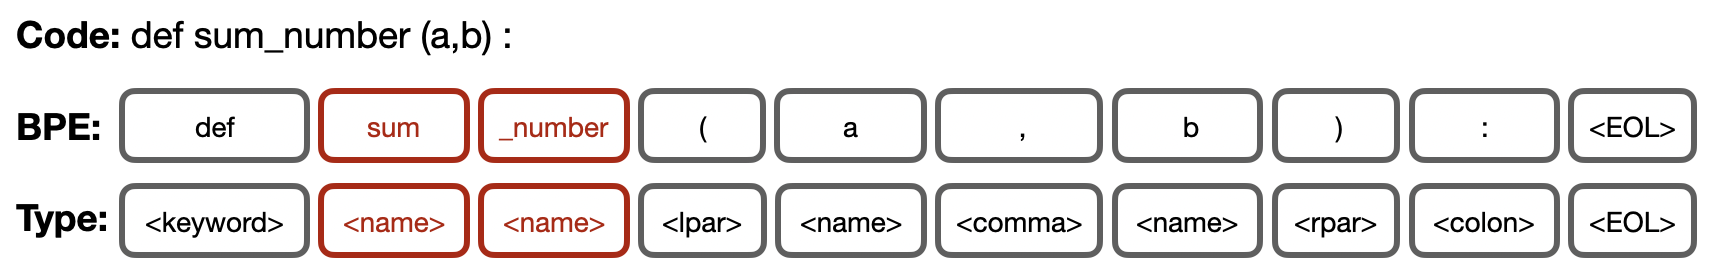
\includegraphics[width=\textwidth/2]{figures/align_dataset.png}
%     \caption{Example of align dataset}
%     \label{fig:align_dataset}
% \end{figure}

%! Author = sbbfti
%! Date = 10/06/2020

% \subsection{Models}
% \textit{finish} \kla{reviewers could argue that some other models learn both syntactic and semantic information. If this model only learns syntactic, how are they going to be accurate? check existing work why they call they learn semantic information and see if ours also learn semantic information or not. Otherwise, we are downtown the claim.}

% \kla{should we talk about two prediction tasks somewhere? Task1=? and Task2=}

\subsection{(Step 4) Multi-Task Training Architectures}
\label{sec:approach-arch}


% On the other hand, training multiple single models on multiple tasks is also possible, but predictions are competing and the multiple sources of information are not jointly learned together, leading to inaccurate predictions.



Our \our~leverages a Multi-Task Training (MTT) paradigm, which is a set of techniques designed to learn multiple tasks, allowing the model to capture multiple sources of information.
Traditionally, deep learning is designed for one single learning objective (e.g., only predicting the next code token), limiting its ability to capture other important and useful sources of information (e.g., syntactic information of source code).
Instead of training a model with one single learning objective, the MTT paradigm aims to provide a generalist model with multiple learning objectives, providing a more robust vector representation.
For our \our~approach, we design the target task to predict the next token, while the supporting task (aka. an auxiliary task or additional related non-target task) is to predict the token type.
In addition, we build three variants of \our, with three different MTT techniques, according to two learning styles~\cite{phang2018sentence} as follows.
% (i.e., \our-Hard, \our-Soft, and \our-IFN)

\subsubsection{Multi-Task Learning (MTL)}

Multi-Task Learning (MTL) is an MTT technique to learn multiple tasks simultaneously instead of learning them separately.
Normally, during the learning process, the model aims to optimize a loss function for one single learning objective.
With the MTL approaches, multiple loss functions are optimized together during the learning process, allowing the MTL-based model to simultaneously learn against multiple objectives and share the knowledge understanding from multiple related sources.
In this paper, we consider two main MTL approaches for Multi-Task Learning (MTL)~\cite{ruder2017overview}, i.e., Hard Parameter Sharing (\our-Hard) and Soft Parameter Sharing (\our-Soft).

For \emph{Hard Parameter Sharing}, the key principle is to train a code completion model against two learning objectives, where the loss functions of the two learning objectives ($L_{code}$ and $L_{type}$) are optimized together within the same model.
Formally, the \our-Hard model aims to minimize the following loss function: 
\begin{equation}
    \label{eq:1} 
    \begin{aligned}
    \medmath{L_{Hard} = \argmin_{\omega}(L_{code}(d_{code}, \omega) + L_{type}(d_{type}, \omega))}
    % loss_{hardShare} = codeLoss + typeLoss
    \end{aligned}
\end{equation} 

\noindent , where $d_{code}, d_{type}$ denotes the code token dataset and the token type dataset, respectively, and $\omega$ denotes a model's parameters.
With Hard Parameter Sharing, the weights and model parameters are shared between tasks, allowing the model to explicitly learn the input representations between tasks (i.e., code and type vectors) that are closely related.



% via the shared layers which may help enhance the effectiveness of the target task's results.
% After the shared layers, usually there are separated task-specific output layers for each task.
% However for our work, the tasks have similar outputs i.e. tokens from the vocabulary.
% Therefore, we train both target task and supporting task in the same model simultaneously without separated output layer.

% SynComp hard parameter sharing uses one GPT-2 model with two losses: code prediction loss ($L_{code}$) and type prediction loss ($L_{type}$).
% The model minimize the summation of losses shown in Equation~\ref{eq:1}.



% For hard parameter sharing, the tasks will share the same model backbone which mean the weights and parameter of the model being shared together.
% Only the task-specific output layer that might be different.
% A hard parameter sharing model is one of the most popular multi-task learning techniques.
 

% \kla{wannita will write soft....}

% \subsubsection{MTL: Soft Parameter Sharing Model}
% For soft parameter sharing, each task will have its own model backbone, i.e. separate weights and parameters.
% However, the models are loosely connected by the constraint which try to minimize the distance of the model parameters' difference.
% This is to regularize the model parameters to be similar.
For \emph{Soft Parameter Sharing}, the key principle is similar to Hard Parameter Sharing where the goal is to train a code completion model with two learning objectives.
However, instead of training a model against two tasks like the Hard Parameter Sharing model, the Soft Parameter Sharing is designed to train two individual models for each task ($L_{code}$ and $L_{type}$), allowing each model to learn separately for each task.
Therefore, each learning objective has an individual model (i.e. separated weights and parameters between the learning objectives).
% to learn and predict outputs; 
To allow the model to share the knowledge between tasks (i.e., to learn the similarities between the related parameters), a shared loss function is also used, which is computed as follows:

\begin{equation}
    \label{eq:norm}
    L_{sharing}(\omega_1, \omega_2) = 
    % ||W||_F = 
    \sqrt{\sum_{i=1}^{I}\sum_{j=1}^{J}|\omega_{1(i,j)}-\omega_{2(i,j)}|^2}
\end{equation}

% Nonetheless, the models are loosely connected by the constraint to encourage similarities between related parameters.


% The constraint ($L_{sharing}$) which is used to optimize the difference of distance between the models parameters' applies with Frobenius norm:

\noindent , where $\omega_n$ denotes the model parameters of the  learning objective $n$. Finally, the \our-Soft model aims to minimize the following loss function:

\begin{equation}
\label{eq:2}
\begin{aligned}
    L_{Soft} = \argmin_{\omega_1, \omega_2}
    &( L_{sharing}(\omega_1, \omega_2)\\ 
    &+ L_{code}(d_{code}, \omega_2)\\
    &+ L_{type}(d_{type}, \omega_1))
\end{aligned}
\end{equation}

With Soft Parameter Sharing, each learning objective has its own model parameters and weights, allowing the models to implicitly learn the input representations that might have more connection to a specific task.

% SynComp soft parameter sharing uses two GPT-2 models with three losses: code prediction loss, type prediction loss, and sharing loss. The model minimize the summation of losses shown in Equation~\ref{eq:2}.

\subsubsection{Intermediate Fine-Tuning (IFT)}

\emph{Intermediate Fine-Tuning (IFT)}~\cite{phang2018sentence} adapts a transfer learning concept (i.e., pre-training then fine-tuning) where the goal is to learn multiple tasks sequentially. First, the model is fine-tuned on the supporting task (token type prediction) followed by the target task (code token prediction), respectively.
Thus, the fine-tuned step on the supporting task can be considered the second stage of the model pre-training.
Therefore, the Intermediate Fine-Tuning (IFT) model (\our-IFT) is first trained based on an intermediate self-supervised task (token type prediction), then trained on the target task (code token prediction), allowing the model to gain knowledge on the token type prior to predicting the next code tokens.


\subsection*{GPT-2 Model Architecture}

Among the three variants of the MTT techniques (i.e., \our-Hard, \our-Soft, and \our-IFT), we use the GPT-2 architecture as a base model.
GPT-2~\cite{radford2019language} is a decoder-only Transformer model.
The GPT-2 architecture for code completion consists of three main components: the embedding layer, the decoder block, and the language model head. 
First, the embedding layer embeds the input tokens into vectors with positional encoding, allowing the model to learn the semantic meaning and the position of each code token.
Then, the embedding vectors are fed into the decoder block which contains decoder layers.
Each decoder layer includes masked self-attention layers, feed-forward neural network layers, and normalization layers.
%  It basically always scores the future tokens as 0 so the model can’t peak to future words
The masked self-attention layer indicates which tokens to focus on, while the masking approach prevents the attention mechanism~\cite{vaswani2017attention} to see the unseen tokens in the future.
% \kla{wannita will do the rest}.
% Feedforward neural nets are complex network made up an input layer that accepts information, hidden layers that capture the hidden correlations between each data point, and an output layer which transmit information.
The feed-forward neural network layer is a sophisticated network with hidden nodes to capture the related information between each data point.
% Layer normalization (LayerNorm) is a technique to normalize the distributions of intermediate layers. It enables smoother gradients, faster training, and better generalization accuracy.
The normalization layer makes the learning process more effective by enabling smoother gradients and generalized accuracy.
% The linear layer takes the output of the last decoder block and converts it to a vector whose dimensions are vocabulary size by 1. In short, it takes a lot of inputs and produces a list where each spot represents a token. The higher the number in the spot the better the chance that that token is the best pick. Softmax converts the output of the linear layer to a probability distribution
After $L$ layers of decoder, an output of the last layer is fed to the language model head, i.e. a linear layer, which converts the output to a vector whose dimensions are the same as the vocabulary size.
Lastly, the vector is converted to a probability distribution by the softmax activation function.
Formally, to predict the next token $x_t$ based on a given input sequence, GPT-2 can be represented as follows:

\begin{equation}
\begin{aligned}
    \label{eq:transformer}
    h_0 &= W_e \cdot C + W_p \\
    % \label{eq:transformer2}
    h_l &= decoder\_layer(h_{l-1}), \forall l \in [1,L] \\
    % \label{eq:transformer3}
    P(x_t) &= y_t = softmax(h_n \cdot W^T_e), t \in [0, N]
\end{aligned}
\end{equation}

\noindent, where $W_e$ is the tokens embedding matrix, $C$ denotes the context vector of tokens, $W_p$ is the position embedding matrix, $L$ is a number of decoder layers, and $N$ is the length of the sequence.
We follow the traditional language models by maximizing the log-likelihood of:

\begin{equation}
    \label{eq:log-likelihood}
    L(x_t) = \sum_i{\log P(x_i|x_1...x_{i-1}, \omega)}
\end{equation}

\noindent, where $\omega$ is the model parameters that are learned during the optimization process.
Particularly, \our~uses the pre-train CodeGPT~\cite{lu2021codexglue} that is pre-trained on the CodeSearchNet dataset~\cite{husain2019codesearchnet} as a starting checkpoint.


% Below we provide details for each training techniques.



% In Fig.~\ref{fig:overview} shows the architectures of all described models.
% During the training phase, both tasks are cooperatively trained; however, the task can separately predict in the inference phase as shown in Fig.~\ref{fig:overview}.
% In other words, the token type information is used only to support throughout the training phase requiring no token type extraction in the inference phase.
% which yield to the benefit of on-the-fly model by not requiring token type extraction in the inference phase.

% SynComp has GPT-2~\cite{radford2019language}, a Transformer decoder-only model, as a based model for all techniques.
% The based model consist of three main components: embedding layer, decoder block, and language model head. 
% Before handing that to the first block in the model, we need to incorporate positional encoding – a signal that indicates the order of the words in the sequence to the transformer blocks.



% \gls{ifn} is adapted from transfer learning paradigm which is about pre-training and then fine-tuning on target task.
% Specifically, this is the training technique for sequential training.
% The model is fine-tuned on supporting tasks and then target task respectively.
% This technique benefit the model to learn the second stage of pre-training with intermediate supervised task that might mitigate the brittleness and improve the robustness and performance of the target task~\cite{phang2018sentence}.

% In our case, SynComp intermediate fine-tuning uses one GPT-2 model with the token type prediction as the supporting task. 
% Thus, we first fine-tune our \gls{ifn} model on type dataset.
% Then we fine-tune the same model again on code prediction task.




% Recently, both MTL approaches are used in code completion.
% For example, Liu~\ea~\cite{liu2020self, liu2022unified, liu2020multi} leverage Hard Parameter Sharing, while CodeFill~\cite{izadi2022codefill} leverage Soft Parameter Sharing.




% Typically, there are two approaches for training \gls{mtl}: hard parameter sharing and soft parameter sharing~\cite{ruder2017overview}.

% Basically, the inspiration to train the tasks at the same time on one or many models with jointly conditions.
% On the other hand, \gls{ifn} is the model training technique for \emph{sequential} training.

% Specifically, the model is fine-tuned sequentially on each supporting tasks, and then the target task respectively~\cite{phang2018sentence}.

% \subsubsection{Intermediate Fine-Tuning}

% To achieve this, we consider the following three MTT training techniques~\cite{phang2018sentence}.




% Some code completion research starts to apply \gls{mtl} with different tasks and datasets~\cite{izadi2022codefill, liu2020self, liu2022unified, liu2020multi}.
% Particularly, most of the time \gls{mtl} has been used for \gls{ast} training~\cite{izadi2022codefill, liu2020self, liu2022unified} in order to learn syntactic information of source code.
% However, the source code of code completion task is usually incomplete or syntactically incorrect which leads to the limitations of extracting \gls{ast} data in practice (section 2.2).
% To address the limitations of previous works, our work
% % is the first to
% leverages \gls{mtl} with \emph{token type} information that represent the light-weight syntactic information and is more flexible to be extracted. 
% Moreover, although showing benefits in many NLP research~\cite{phang2018sentence, weller2022use, gururangan2020don}, to the best of our knowledge \gls{ifn} has never been introduced to code completion field.
% Therefore, this motivate us to include the technique to our experiment along with \gls{mtl}.







% PyCoder-Hard
% PyCoder-IFT

% However, sometimes the additional related non-target tasks (i.e. supporting task or auxiliary task) are presented with the intention of improving the target task's performance.
% When supporting task has been presented during the fine-tuning stage, there are multiple techniques to combine or alternate between these target task and supporting task -- such techniques can be called \emph{multi-task training techniques}.


% at the same time rather than separately.

% target dataset
% supporting dataset



% In the past, pre-train language model and fine-tune on target task has become the standard paradigm for NLP~\cite{raffel2020exploring} and also be adapted to many tasks in software engineering~\cite{wang2021codet5, feng2020codebert}.

% These kind of tasks are called supporting task or auxiliary task.
% However, when non-target tasks has been presented more than one


% Recently in NLP, there is a study for how to best make use of the supporting data~\cite{weller2022use}.
% Two predominant methods used are \gls{mtl} and \gls{ifn}. 
% \gls{mtl} is a model training technique for \emph{simultaneous} training.
% Typically, there are two approaches for training \gls{mtl}: hard parameter sharing and soft parameter sharing~\cite{ruder2017overview}.
% Basically, the inspiration to train the tasks at the same time on one or many models with jointly conditions.
% On the other hand, \gls{ifn} is the model training technique for \emph{sequential} training.
% Specifically, the model is fine-tuned sequentially on each supporting tasks, and then the target task respectively~\cite{phang2018sentence}.



% \subsubsection{MTL: Hard Parameter Sharing Model}
% For hard parameter sharing, the tasks will share the same model backbone which mean the weights and parameters of the model being shared together.
% Only the task-specific output layer that might be different.
% A hard parameter sharing model is one of the most popular multi-task learning techniques.
% This technique completely shares the model backbone (i.e. weights and parameters) between tasks.
% The benefit is that the model could \emph{explicitly} learn the input representations between tasks via the shared layers which may help enhance the effectiveness of the target task's results.
% After the shared layers, usually there are separated task-specific output layers for each task.
% However for our work, the tasks have similar outputs i.e. tokens from the vocabulary.
% Therefore, we train both target task and supporting task in the same model simultaneously without separated output layer. 

% SynComp hard parameter sharing uses one GPT-2 model with two losses: code prediction loss ($L_{code}$) and type prediction loss ($L_{type}$).
% The model minimize the summation of losses shown in Equation~\ref{eq:1}. where $d_{code}, d_{type}$ denotes code and type dataset respectively, and $\omega$ denotes a model's parameter.


% \begin{equation}
%     \label{eq:1} 
%     \begin{aligned}
%     \medmath{L_{hardShare} = \argmin_{\omega}(L_{code}(d_{code}, \omega) + L_{type}(d_{type}, \omega))}
%     % loss_{hardShare} = codeLoss + typeLoss
%     \end{aligned}
% \end{equation} 

% \subsubsection{MTL: Soft Parameter Sharing Model}
% For soft parameter sharing, each task will have its own model backbone, i.e. separate weights and parameters.
% However, the models are loosely connected by the constraint which try to minimize the distance of the model parameters' difference.
% This is to regularize the model parameters to be similar.
% A soft parameter sharing model has particular model backbones for each objective task, i.e. separated weights and parameters.
% Each model learns and predicts results nearly independently; to be precise, there are loosely connected by the constraint to encourage similarities between related parameters.
% More specifically, the model is trained on each task individually along with penalizing on the distance between the model parameters' difference.
% The benefit of this technique is that each task has its own model parameters, so the model \emph{implicitly} learn the input representations and might have more connection to a specific-task.
% This constraint is expressed as \emph{sharingLoss} ($L_{sharing}$). 
% In this work, we apply the square Frobenius norm in Equation~\ref{eq:norm} as the \emph{sharingLoss}.

% \begin{equation}
%     \label{eq:norm}
%     ||W||^2_F = \sum_{i=1}^{I}\sum_{j=1}^{J}|w_{i,j}|^2
% \end{equation}

% SynComp soft parameter sharing uses two GPT-2 models with three losses: code prediction loss, type prediction loss, and sharing loss. The model minimize the summation of losses shown in Equation~\ref{eq:2}.
% \begin{equation}
% \label{eq:2}
% \begin{aligned}
%     L_{softShare} = \argmin_{\omega_1, \omega_2}
%     &( L_{sharing}(\omega_1, \omega_2)\\ 
%     &+ L_{code}(d_{code}, \omega_2)\\
%     &+ L_{type}(d_{type}, \omega_1))
% \end{aligned}
% \end{equation}

% \begin{equation}
%     \label{eq:2}
%     loss = \alpha * codeLoss + \beta * typeLoss + (1 - \alpha - \beta) * sharingLoss
% \end{equation}

% \subsubsection{STILTs: Intermediate Fine-tuning}
% From pre-training on supporting task, and then fine-tuning on the target task;
% this training technique apply the same paradigm method but with many supporting tasks called auxiliary tasks.



% \kla{move from background / will revise later}
% \emph{SynComp} leverages a multi-task training model, focusing on two training tasks: source code prediction (semantics information), and token type prediction (syntactic information).
% While the code prediction is a target task, the type prediction is a supporting task.
% SynComp explores on 3 multi-task training techniques: (3.4.1)~MTL: Hard Parameter Sharing Model, (3.4.2)~MTL: Soft Parameter Sharing Model, and (3.4.3)~\gls{ifn}: Intermediate Fine-tuning Model.
% Supplementary Training on Intermediate Labeled-data Tasks Model.



% Therefore, the training phase consist of 2 tasks: source code prediction and token type prediction.
% There are multiple techniques to learn such target task (source code prediction) with auxiliary task (type prediction). However, SynComp is inspired by weller~\ea~\cite{weller2022use} to leverage the usage of \gls{mtl} and \gls{ifn} training techniques. 

% \kla{why these three types are chosen? why do we need to explore these? - could cited~\cite{weller2022use} in the previous paragraph be the reason?}

% There are two dominant approaches in \gls{mtl} which are \emph{(3.3.1) hard parameter sharing model} and \emph{(3.3.2) soft parameter sharing model}. The core idea of both techniques is to learn the hidden robust representations from related tasks.

% \textbf{\gls{gtt}}
% We have 2 objective tasks here. First, the main task is code prediction and second task is type prediction as the auxiliary task. Both tasks, the models learn to predict in single-token level. Therefore when using in token-level prediction, the model can be used directly. For line-level prediction, the models are the same as in token-level prediction, however, are set to prediction until stop criteria is reached.


% \textit{finish} \kla{it would be great if we can discuss the advantages/disadvantages of each model? why we use them? why others are not explored? how are they different? }

% \textit{finish} \kla{I think we haven't talked about CodeGPT yet. Why using CodeGPT, instead of GPT-2? What is the limitation of CodeGPT? }
% We decide to include this method because the evidence shows that \gls{ifn} and \gls{mtl} are competitive and useful in some different scenario. If auxiliary task is larger than the target task, \gls{ifn} tend to perform better than \gls{mtl} \cite{weller2022use}. However, our type dataset is smaller than code dataset due to the tokenization process which all types are added in as the special tokens (see session 4.2). But we still choose to train \gls{ifn} in order to test the argument on the code completion task. We don't use repeated type dataset (see session 4.1) because dissimilar to \gls{mtl}, \gls{ifn} doesn't train code and type prediction simultaneously so we would like to maintain the granularity of data as normal.

% \begin{figure}[]
%     \centering
%     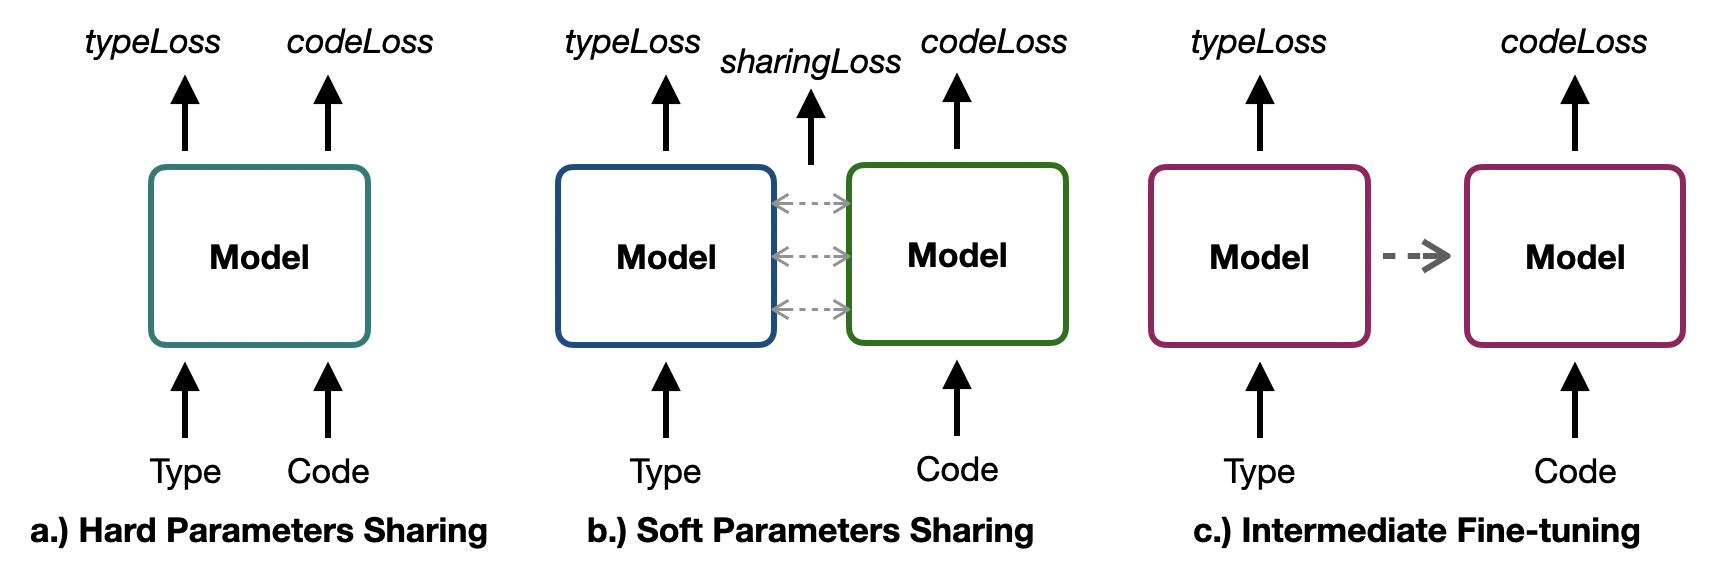
\includegraphics[width=\columnwidth]{figures/model_arch.png}
%     \caption{Model architectures (tentative pic)}
%     \label{fig:arch}
% \end{figure}

\subsection{(Step 5) Hyperparameter Task Weighting}
\label{sec:approach-weight}

Since our \our~leverages MTL training techniques to learn multiple different tasks simultaneously, some tasks may have a higher influence than others, which later may produce an unsatisfactory accuracy for the other tasks (called a conflicting gradient problem).
To prevent such conflicting gradients between tasks, it is important to find the most optimal task weights by minimizing the loss.
Therefore, we optimize the hyperparameters ($\alpha_i$) to adjust the task weights to find optimal task weights for our architecture.
Specifically, we aim to minimize the loss of the code prediction task along with the type prediction task using the following loss function.

\begin{equation}
    \label{eq:rq3}
    L_{MTL} = \argmin_{\omega}(\sum_{i}\alpha_i \cdot L_{i}(d, \omega))
    % L_{MTL} = \min_{\omega}(\alpha * L_{code}(\omega) + (1 - \alpha) * L_{type}(\omega))
    % loss = \alpha * codeLoss + (1 - \alpha) * typeLoss
\end{equation} 

% \our~performs a static weighted linear sum of losses which fixed the task's weights throughout the training phase.
% In Equation.~\ref{eq:rq3} presents SynComp's task weighing formula where $\alpha$ is the hyperparameter weight. 

\subsection{(Step 6) Decoding Methods}
\label{sec:approach-decoding}

Decoding is a method to select the next token from the potential vocabulary when generating a sequence.
Although selecting only the highest probable token is suitable for a single step, it might be a sub-optimal for the sequence.
Since the search space of the next tokens is large, different decoding methods will have different mechanisms, providing different predictions of the next tokens.
Thus, the selection of the decoding methods may have an impact on the overall performance of our ~\our.
In the code completion literature, we found that Beam Search is one of the most commonly used decoding methods.
However, Holtzman~\ea~\cite{holtzman2019curious} found that there exist other decoding methods that are widely used in the NLP area, yet remain largely explored in the code completion literature.
Thus, we aim to experiment with the six following decoding methods.

\begin{itemize}
    \item \textbf{Greedy} is a method to select the maximum probable vocabulary to be the next tokens.
    This method assumes that the model already outputs the best probability in every timestep.
    % it generates all possible tokens in the vocabulary list; then, it will choose top B candidates that have the most probability. Those B candidates will move to the next time step, and the process repeats. In the end, there will only be B candidates. The search space is only (10,000)*B.
%     Although selecting only the highest
% probability token is suitable for a specific time step, it
% might be a sub-optimal for a sequence. 
    
    \item \textbf{Beam Search} applies a search algorithm to generate all possible tokens in the vocabulary; then, it selects the top $b$ (i.e., beam size) probable tokens to continue.
    The Beam Search method is one of the most commonly used decoding methods in text generation tasks~\cite{li-etal-2016-deep, wiseman-etal-2017-challenges}.
    % However, Beam Search may not always achieve optimal results, since it does not consider the whole vocabulary, but instead only the top $b$ (i.e., beam size) probable tokens.
    % Nevertheless, Beam Search still performs faster than an exhaustive search.
    
    % ; however, it balances between the performance and the computational time.
    % The method's time complexity is equals to $O(b*V)$ where $V$ is the vocabulary size.
    % It . 
    
    % recommend the most probable $b$ next tokens according to a defined $b$ beam size threshold.

    
    
    
    % by expanding the graph in a limited set called beam~size~($b$).
    % In each timestep, the method generates all possible tokens in the vocabulary; then, it select the top $B$ probability tokens to continue.
      
    
    \item \textbf{Sampling} is a method to randomly select the next token from the actual probability distribution assigned by the model.
    Different from Greedy and Beam search methods which in some cases may recommend only the same probable next tokens at different timesteps, the sampling method may recommend different next tokens at different timesteps (i.e., non-deterministic).
    % We put the sampling method in this study as the baseline for other decoding methods. All of the methods that required sampling are set the seed value to the same number.
    
    % Temperature is used to increase the probability of probable tokens while reducing the one that is not. Usually, the range is 0 < temp ≤ 1. Note that when temp=1, there is no effect.
    \item \textbf{Sampling with Temperature} applies a temperature parameter to shape the probability distribution~\cite{ackley1985learning}, which is different from the original sampling method where the randomness is arbitrary.
    The temperature is used to increase the probability of the most probable next tokens, while decreasing the probability of the others.
    We note that the probability of the least probable next tokens is only decreased, but they are not removed from the recommendation.
    The range of the temperature value is usually at $0 < temp \le 1$, where $temp = 1$ is a normal sampling.

    % Additional to normal sampling which could be arbitrary, sampling with temperature method 
    \item \textbf{Top-K Sampling} aims to truncate the probability distribution by choosing the top-$k$ probable next tokens from the vocabulary, then, re-scale the distribution and perform sampling based on the new distribution.
    This method ensures that the less probable next tokens will not be generated, while only the top-$k$ probable next tokens are only considered during the sampling process.
    
    \item \textbf{Top-P Sampling (Nucleus Sampling)} is similar to the Top-k sampling method where the Top-P sampling method also truncates the probability distribution, but with different criteria. 
    Top-P sampling prunes the distribution by the cumulative probability of the current step $\ge p$~\cite{holtzman2019curious}; then, re-scale and perform sampling.
    Formally, given the probability P, we can define the smallest summation of the probability as $V_p$ in
    \begin{equation}
        \label{eq:top-p}
        \sum_{x\in V_p} P(x|x_{1:i-1}) \ge p
    \end{equation}
    The benefit of this method is that it can dynamically adjust the number of $k$ depending on the certainty of the model.
    If the model is very certain on some tokens, the search space is small, and vice versa.
\end{itemize}

%  the decoding method defines the way the system handles its search space over potential output utterances when generating a sequence
% The result performance in code completion may not depend only on the model, but also a method to select the output tokens from the probability distribution, i.e. a decoding method.
% The decoding method defines the way to handle the search space over potential output tokens when generating a sequence.
% Although selecting only the highest probability token is suitable for a specific time step, it might be a sub-optimal for a sequence.
% Therefore, various alternative way for decoding methods is proposed in NLP field; however, there is still a limited exploration in code completion which is similar to text generation field.
% Thus, we select 6 following decoding methods to study in this work in order to seek for the best use of our architecture.

% Even though the model leverages the token type prediction as the supporting task during the training process, at the inference phase, the model will perform only the code token prediction.
% Thus, the token type information is not required at the inference phase, allowing our \our~to perform on-the-fly code completion.



\subsection{(Step 7) Code Completion}
\our~performs predictions at two granularity levels, i.e., at the token level and at the line level.

\textbf{Token-level code completion} is a process to predict the next token (the right side), given the prior code tokens as a context (the left side).

\textbf{Line-level code completion} is similar to the token-level prediction, but the model aims to predict the next tokens until completing the whole line of code (i.e., not just only one single next token).
For the line-level prediction, we leverage the same model used for the token-level code completion task to iteratively generate the next token, where the newly generated token is used as a context for the next step of the prediction.
This process is repeated iteratively until the model generates a $\langle EOL \rangle$ token, or until it reaches a certain $n$ threshold ($n=100$, following the CodeXGlue~\cite{lu2021codexglue}).




% is occurred or the number of generated tokens become specific \emph{n} tokens, has been reach. In this work \emph{n} is set to 100.


% The task is to complete an unfinished line of code.
% Instead of training a new model, \our~adapts the token-level model for line-level prediction using a following process.
% There are 3 main steps for line-level prediction process: 1.) the model predict the next token; 2.) the predicted token is concatenated to the previous left-side context; 3.) the new sequence is recursively fed back to the model to predict the next new token.
% Firstly, the model predict the next token.
% Then, the predicted token is concatenated to the previous left-side context, and recursively fed back to the model to predict the next new token.
% This procedure performs until either one of the stop conditions, which are generating until tokens $\langle EOL \rangle$ is occurred or the number of generated tokens become specific \emph{n} tokens, has been reach. In this work \emph{n} is set to 100.
% The two stop conditions for line-level prediction are generating until tokens $\langle EOL \rangle$ is occurred, or the number of generated tokens reach n tokens.
% line-level tokens by recursively inputting the concatenation of the left-side context and the generated code.


% Specifically, as shown in the inference phase in Fig.~\ref{fig:overview}, the model receive only source code as an input in order to perform the code completion.
% Thus, \our~which has already learnt syntactic information do not need token type data for inferring, and able to remain the ability of \emph{On-the-Fly} code completion. 



